\documentclass[12pt, twoside]{article}
\usepackage{jmlda}
\usepackage[]{algorithmic}
\usepackage{graphicx}
\newcommand{\hdir}{.}

\begin{document}

\title
    [] % краткое название; не нужно, если полное название влезает в~колонтитул
    {Условия существования петель скрытой обратной связи в рекомендательных системах}
\author
    [А.\,А.~Пилькевич] % список авторов (не более трех) для колонтитула; не нужен, если основной список влезает в колонтитул
    {А.\,А.~Пилькевич, A.\,C.~Хританков} % основной список авторов, выводимый в оглавление
    [А.\,А.~Пилькевич$^1$, A.\,C.~Хританков$^2$] % список авторов, выводимый в заголовок; не нужен, если он не отличается от основного
\email
   {anton39reg@mail.ru; anton.khritankov@gmail.com}
%\thanks
%    {Работа выполнена при
%     %частичной
%     финансовой поддержке РФФИ, проекты \No\ \No 00-00-00000 и 00-00-00001.}
%\organization
%    {$^1$Организация, адрес; $^2$Организация, адрес}
\abstract
  {В работе исследуется эффект  петель скрытой обратной связи в рекомендательных системах.
  Под положительной обратной связью подразумевается неограниченный рост интереса пользователя к предлагаемым объектам. 
  Решается задача поиска условий возникновения положительной обратной связи для системы c алгоритмом Thomson Sampling Multi-armed Bandit с учётом наличия шума в выборе пользователя.
  В задачах без шума известно, что существуют условия неограниченного роста. 
  Но отсутствие не реализуются в реальных системах.
  Экспериментально проверяются полученные условия в имитационной модели.

\bigskip
\noindent
\textbf{Ключевые слова}: \emph {machine learning; hidden feedback loops; echo chamber; filter bubble}
}
%данные поля заполняются редакцией журнала
\doi{}
\receivedRus{}
\receivedEng{}

\maketitle
\linenumbers
\section{Введение}
Рекомендательные системы являются важной составляющей социальных сетей, веб-поиска и других сфер [...]. 
Рассматривается эффект петель скрытой обратной связи, который подразумевает рост качества предсказаний, как результат учёта принятых решений. 
Эффект петель скрытой обратной связи в реальных и модельных задачах в  публикациях [...] описыается как нежелательное явление. 
Частные и часто рассматриваемые случаи скрытой обратной являются echo chamber и filter bubles [1].
До сих пор нет какой-либо строгой формализации условий возникновения этих эффектов при условиях приближенных к реальности. 

Целью данной работы является нахождение условий существования петель обратной связи в рекоммендательной системе с алгоритмом Thomson Sampling в условиях зашумлённости выбора пользователя.
Зашумлённость выбора рассматривается, как смещение первоночального интереса к исходному объект или категории.
Предлагается способ отыскание условий модели исходя из теоретических свойств алгоритма TS. 
Для описания условия предлагается рекуретного соотношения для регардов.  
Также рассмаривается вариант нахождения этих условий чисто из экспериментов. 
Наибольший интерес представляет матетическое описание искомых условий с дальнейшим экспериментальным подтверждением полученных условий.
Для проверки результатов используется имитационная модель, использующая синтетические данные.  

Уже существует модель [1] этого эффекта в случае отсутствия шума в действиях пользователя, что не реализуется на практике. 
Подобное исследование проводилось в статье [1] на примере различных моделей ( Oracle, Optimal Oracle, UCB,  TS ) в задаче многорукого бандита. 
Им удалось показать условия существования неограниченного роста интереса пользователя. 
В работе [2] изучалась схожая постановка задачи и были получены условия возникновения, но рассматривалась линейная модель и градиентный бустинг. 
Важным отличием данной работы является факт рассмотрения более сложных условий модели, таких как шум в выборе пользователя и другой алгоритм рекомендательной системы.  

\section{Постановка задачи}
\paragraph{Модель рекомендательной системы}
Рекомендательная система выбирает элементы $(a^1, \dots, a^l)$ из конечного набора $M$. 
Обозначим за $t$ очередной момент выдачи рекомендаций.
Истинный $\textit{интерес}$ пользователя к элементу $a \in M$ описывается неизветсной функцией $\mu_t : M \to \mathbb{R}$. 
При этом,  считается, что чем больше значени$\mu_t (a)$, тем заинтересованние пользователь в рекомендции $a$.

После очередного набора рекомендаций $a_t = (a_t^1, \dots, a_t^l)$ пользователь возвращает $\textit{отклик}$ $c_t~= (c_t^1, \dots, c_t^l)$. 
В отсутствие шума в ответах пользователя, он выбирает элементы случайно и независимы, пропорционально $\mu_t(a)$.
Значит отклик будет имеет распределение Бернулли : $c_t^i \sim Bern (\sigma(\mu_t(a_t^i)))$, где $\sigma$~--- сигмойда. 

Потребуем от пользователя, что интерес во времени описывается как $\mu_{t+1} \geq \mu_{t}$, если $c_t = 1$,  $\mu_{t+1} < \mu_{t}$ иначе. 
Тогда эффект обратной связи выражается как $\lim_{t \to \infty} \|\mu_t - \mu_0 \|_2 = \infty$.
Обновление интереса происходит по правилу : 
$\mu_{t+1} - \mu_{t} = \delta_t c_t - \delta_t (1 - c_t)$, 
где $\delta_t \sim U[0, 0.01]$

Оптимизационной задачей рекомендательной системы является минимизация регрета. 
Максимальная сумма ревардов : \[ \max_{c_t^i} \sum_{t = 1}^T \sum_{i = 1}^l c_t^i = T \cdot l.\] 
Тогда задача ставится так : 
\[
  T \cdot l - \sum_{t = 1}^T \sum_{i = 1}^l c_t^i \to \min_{b}, 
\]
где $b$~--- используемый алгоритм в рекомендательной системе. 

\paragraph{Алгоритм}
В данной задаче рекомендательная система будет использовать алгоритм Thompson Sampling для задачи Бернуллиевского бандита.  
Бандитами являются отклики пользователя на очередую рекомендацию, а средним ревардов: $\sigma(\mu_t(a_t^i))$.

В начальный момент времени определены вероятности Бернуллиевских случайных величин для элементов $M$ равные $\pi_0(\theta_1), \dots, \pi_0(\theta_m)$. 
Задаётся априорное распределение для $\theta_i$ равное Бэта распределению $Beta(1, 1) = U[0, 1]$. 
Апостериорное распределение для элемента $a^i \in M$ будет описываться бэта распределением: $Beta(\alpha_t^i, \beta_t^i)$. 
А параметры будут обновляться по закону :
$\alpha_{t+1} = \alpha_t + c_t, \beta_{t+1} = \beta_t + 1 - c_t$.

\paragraph{Учёт шума в поведении пользователя}
Шум откликов будет описываться следующим образом: 
\begin{gather*}
  c_t^i \sim Bern (\sigma(s_t^i \cdot \mu_t(a_t^i) + w \cdot (q_t^i - 0.5))), \\
  P(s_t^i = 1) = p, \\ P(s_t^i = -1) = 1 - p, \\
  q_t^i \sim U[0, 1].
\end{gather*}
Величина $p$ должна быть равна доле шума в ответах. 

Также рассматривается случай марковского процесса: 
\begin{gather*}
  P(s_t^i = 1 | s_{t-1}^i = 1) = \min(1, p + u), \\ 
  P(s_t^i = 1 | s_{t-1}^i = -1) = \max(0, p - u). 
\end{gather*}

\paragraph{Цель}
Целью работы является теоретический анализ условий сходимости TS для различных параметров шума $p, w, u$ и экспериментальное подтверждение полученых соотношений. 
Также делается уточнений условий из [1]. 

\section{Теоретическое обоснование}
При достаточно большом $t$ бандин имеет очень узкое распределение, поэтому точно извествно, что он буде рекомендовать.
Для случая нормы интересов: 
\begin{gather*}
  \|\mu_t - \mu_0 \|^2_2 = \sum_{i=1}^M (\mu_t^i - \mu_0^i)^2,
\end{gather*}
с ростом $t$ сновной вклад будут давать только $l$ объектов.

Тогда рассмотрим поведение интереса для произвольного фиксированного объекта $a \in M$. 
Обновление интереса происходит согласно: $\mu_t - \mu_{t-1} = \delta_t c_t - \delta (1 - c_t)$.

Случайные величины $\delta_j, c_j$ независимы, поэтому: $E \delta_j c_j = E \delta_j E c_j$. 
Для удобства будем считать, что у нас $c_j \sim \text{Bern}_{\pm}$
Тогда: 
\begin{gather*}
  E (c_t | s_t = x, q_t = y) = 2 \sigma(x \cdot \mu_{t-1} + w \cdot (y-0.5)) - 1, \\
  E (E (c_t | s_t, q_t = y)) = p \cdot (2 \sigma(\mu_{t-1} + w \cdot (y-0.5)) - 1) - \\ (1-p) \cdot (2 \sigma(- \mu_{t-1} + w \cdot (y-0.5)) - 1).  
\end{gather*}
Далее для простоты считается, что $\sigma(x) \approx \text{ReLU}(x)$.
Поэтому: 
\begin{gather*}
  E (E (E (c_t | s_t, q_t)|q_t)) = 
    \begin{cases}  
      \mu_{t-1} + w, \text{ при } \mu_{t-1} \geq w /2 , \\
      \frac{1}{w} (\mu_{t-1} +\frac{w}{2})^2 + \frac{w}{2} (1 - (\frac{1}{2} - \frac{\mu_t}{w})^2), \text{ иначе.} 
    \end{cases} 
\end{gather*}

Отсюда можно получить рекурентой соотношение:
\begin{gather*}
\end{gather*}

\section{Вычислительный эксперимент}
\paragraph{Описание данных и работы модели}
Перед началом эксперимента фиксируются следующие параметры : $T$~--- кол-во итераций рекомендательной системы, $|M|$~--- кол-во рассматриваемых объектов для рекомендации, $l$~--- кол-во элементов в одной выдачи. 
Также фиксируются параметры шума $p, w, u$.
Далее случайным образом сэмплируются начальное значение интереса $\{\mu_0^i\}_{i=1}^{|M|}$ и параметры априорного распеределения $\{\alpha_0^i, \beta_0^i\}_{i=1}^{|M|}$  

Генерация элементов очередной рекомендации производится на основе текущего апостериорного распредления. 
Выбираются элементы с наибольшим значением. 
Получение отклика от пользователя заключается в генерации случайных величин на основе рекомендации.
Далее идёт обновление параметров апостериорного распределения по правилу $\alpha_{t+1} = \alpha_t + c_t, \beta_{t+1} = \beta_t + 1 - c_t$, и обновления интереса согласно 
$\mu_{t+1} - \mu_{t} = \delta_t c_t - \delta_t (1 - c_t)$.

Также рассматривается вариант эксперимента, когда рассматривается рандомная модель генерации рекомендации. То есть случайным образом выбираются $l$ элементов для очередной рекомендации. 

В каждый момент выдачи фиксируются значения интереса $\mu_t^i$, сумма откликов $c_t^i$ и параметры апостериорного распределения. 
По полученным данным строятся графики для определения наличия петель скрытой обратной связи.
Как определялось раньше, петля скрытой обратной связи выражается так: $\lim_{t \to \infty} \|\mu_t - \mu_0 \|_2 = \infty$.

\paragraph{Цель}
Целью эксперимента является наблюдение петель скрытой обратной связи для определённых параметров шума. 
Проверяется гипотеза о возникновении петель при параметрах шума, найденных из теоретических соотношений. 
Важной частью эксперимента является сравнения поведений рекомендательной системы с шумом в ответах пользователя и без. 

\paragraph{Псевдокод}
\begin{algorithmic}
  \STATE Инициализируем $\mu_0^i, \alpha_0^i, \beta_0^i$.
  \FOR{$t$ от $1$ до $T$} 
    \STATE $r_t \leftarrow$ РекомендацияTS()
    \STATE $c_t \leftarrow$ ГенерацияОткликаПользователя($r_t$)
    \STATE ОбновлениеПараметровTS($c_t$)
    \STATE ОбновлениеИнтересаПользователя($c_t$)
    \STATE Сохранение($t, c_t, \mu_t$)
  \ENDFOR
\end{algorithmic}

\section{Результаты}
При определённом диапазоне параметров шума удалось про наблюдать эффект неограниченного роста интереса. 
Наличие петель скрытой обратной связи иллюстрируется следующим графиком: 
\begin{center}
  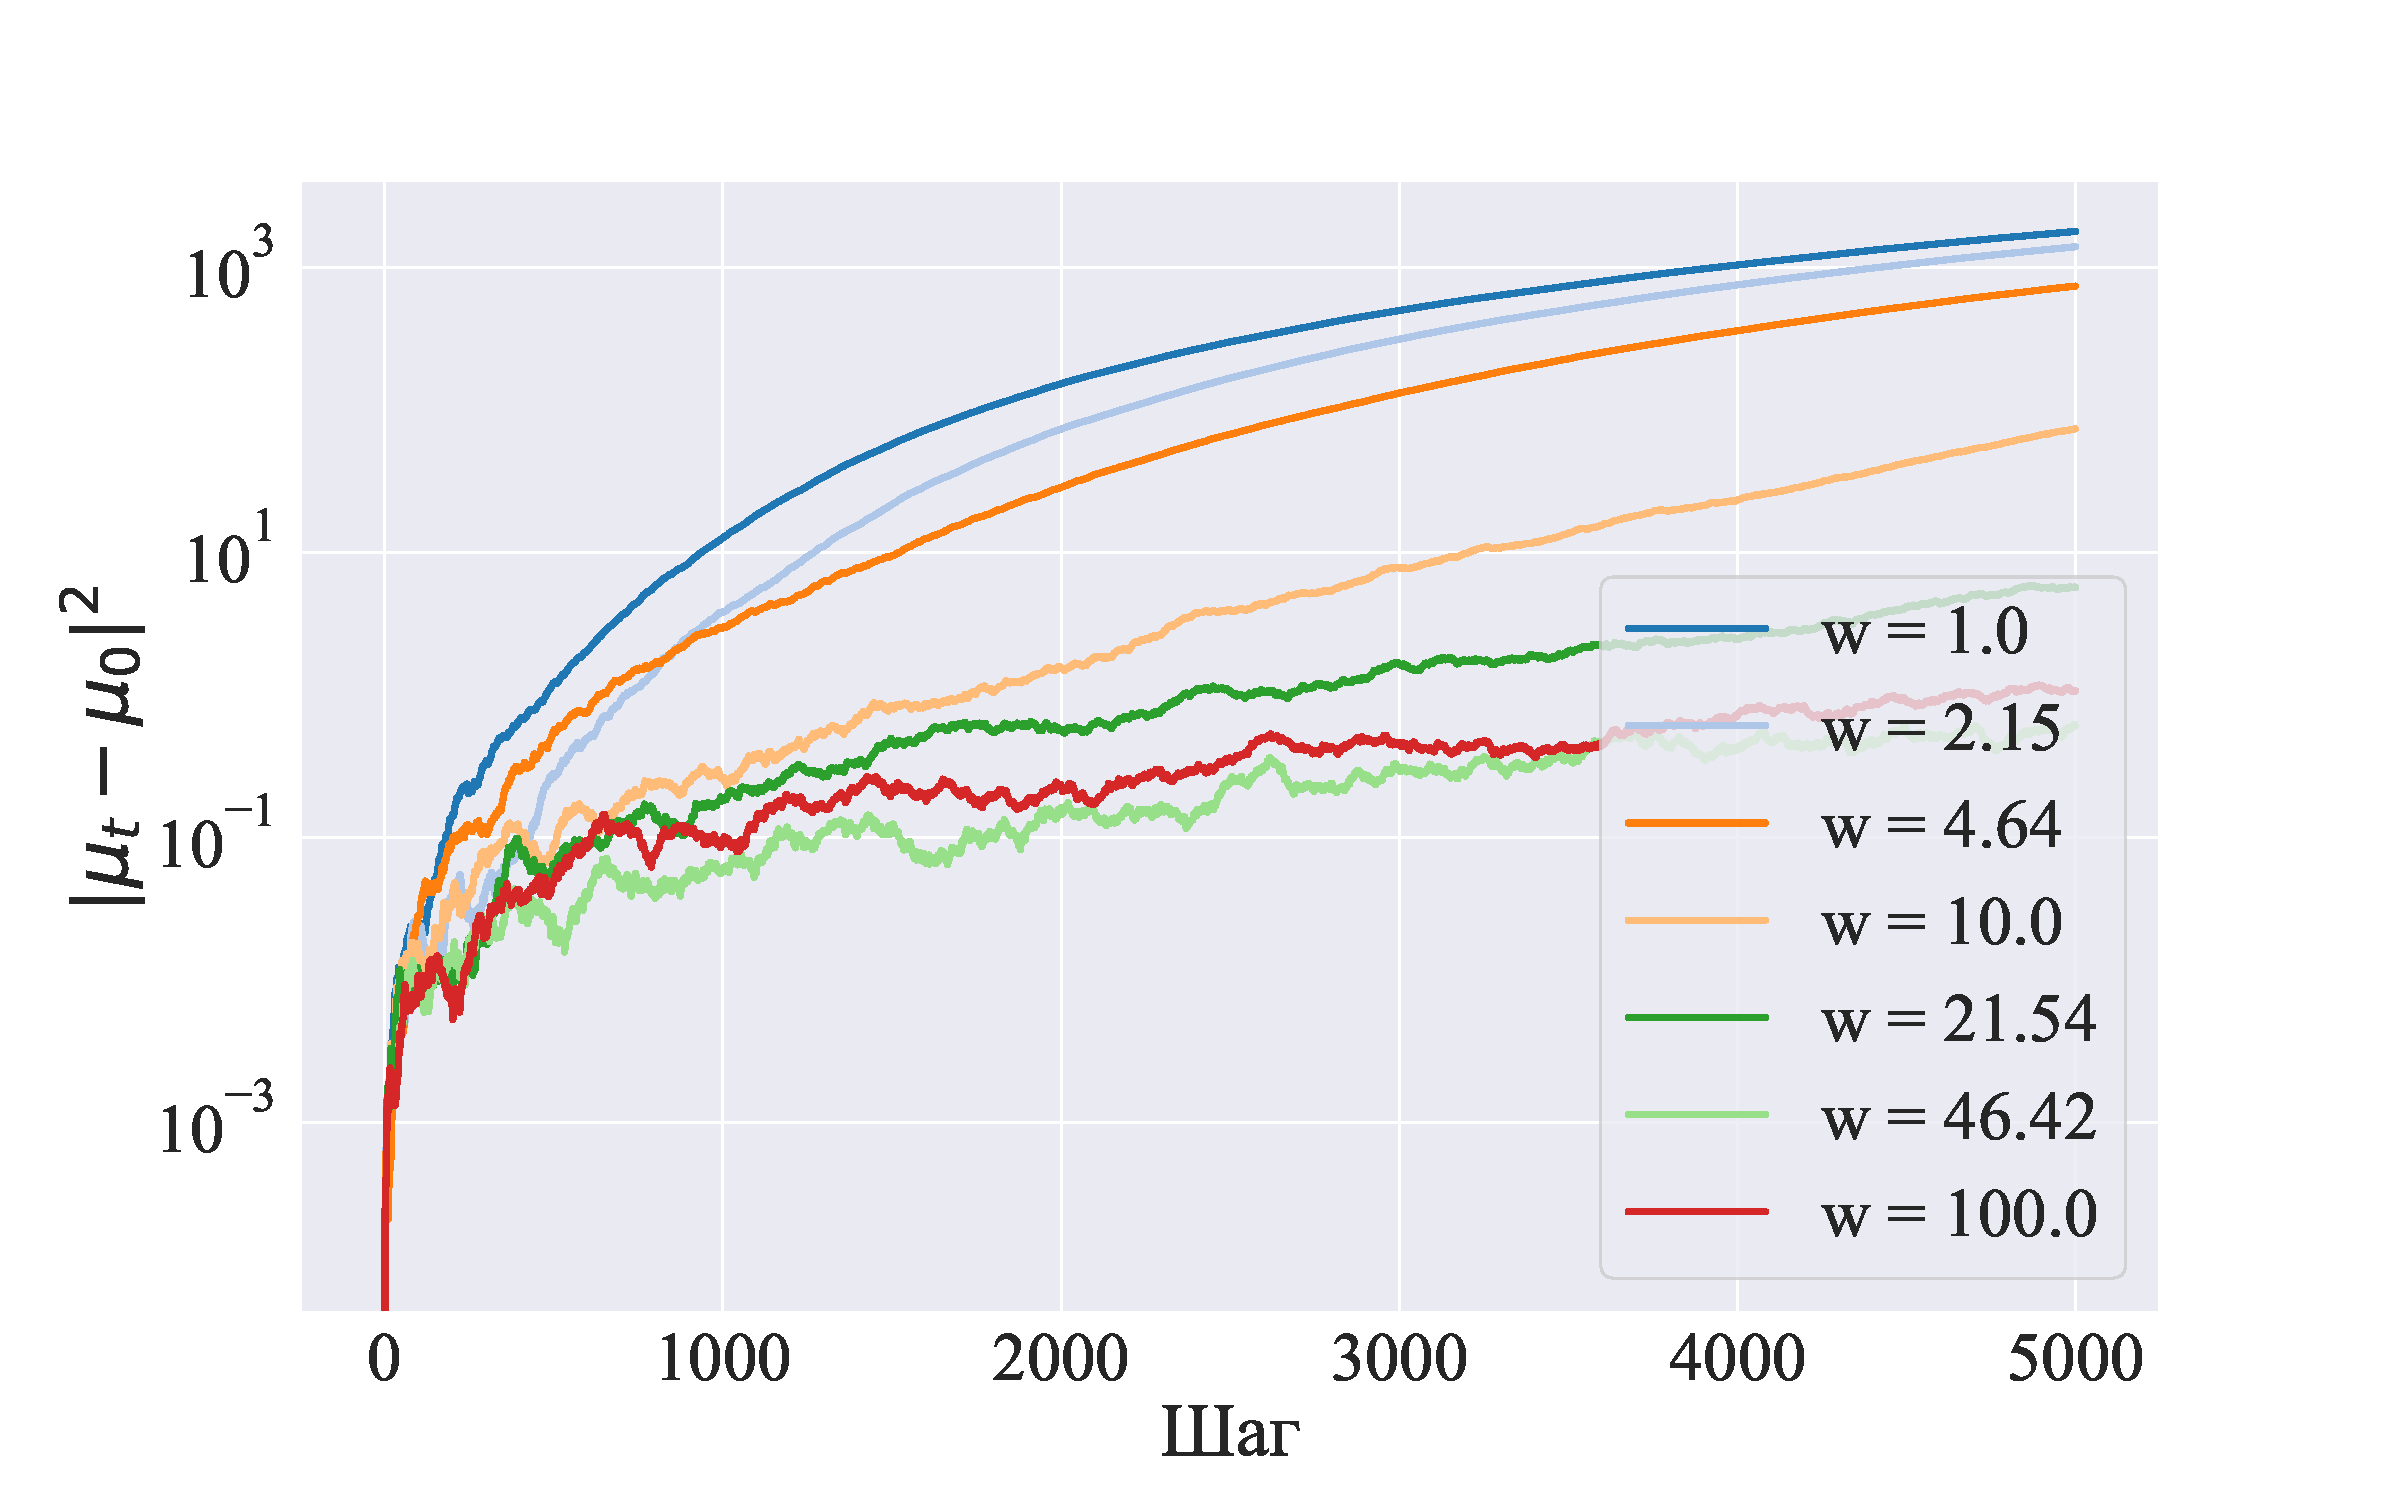
\includegraphics[width=16cm]{norm_interest.pdf}
\end{center}
Как видим, это согласуется с определением петель. 

Из графика суммы ревардов видим, что с определённого момента кривые начинают идти параллельно максимально возможной сумме. 
Это также свидетельствует о наличии петель обратной связи. 
\begin{center}
  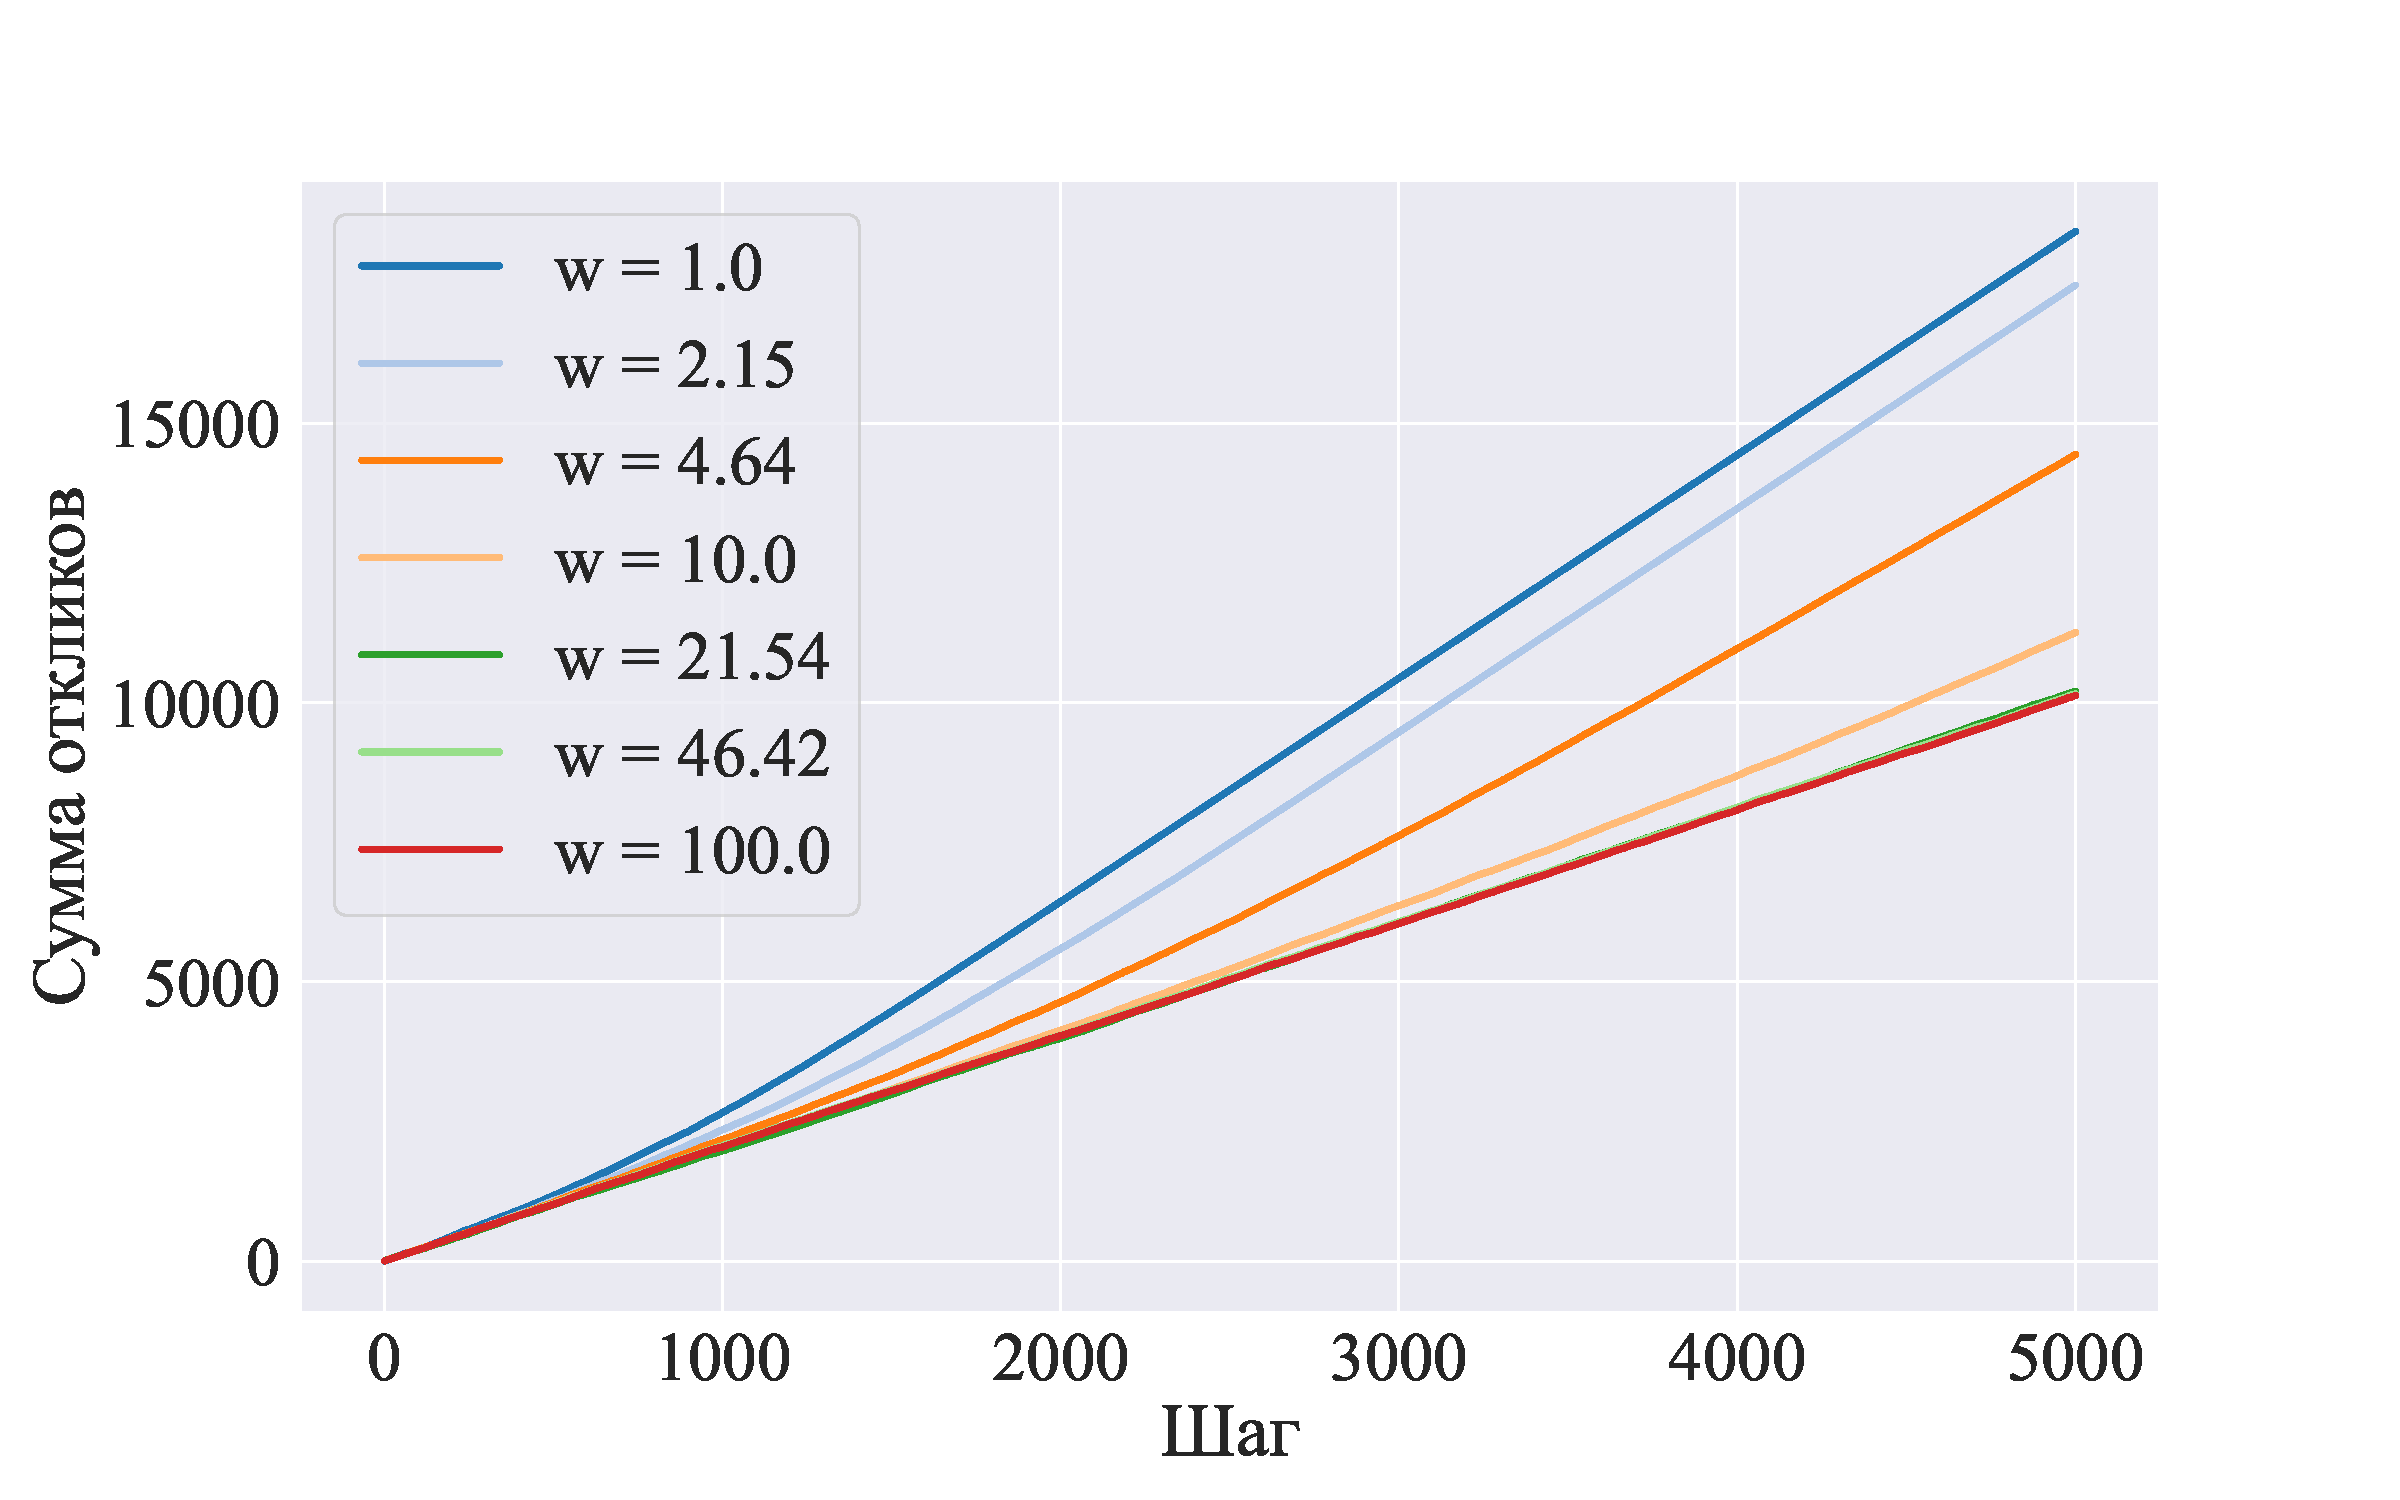
\includegraphics[width=16cm]{rewards.pdf}
\end{center}

Для случайной модели не наблюдается явного образования петли. 
Она более хаотична и отстутствует тренд неограниченного роста интереса.   
\begin{center}
  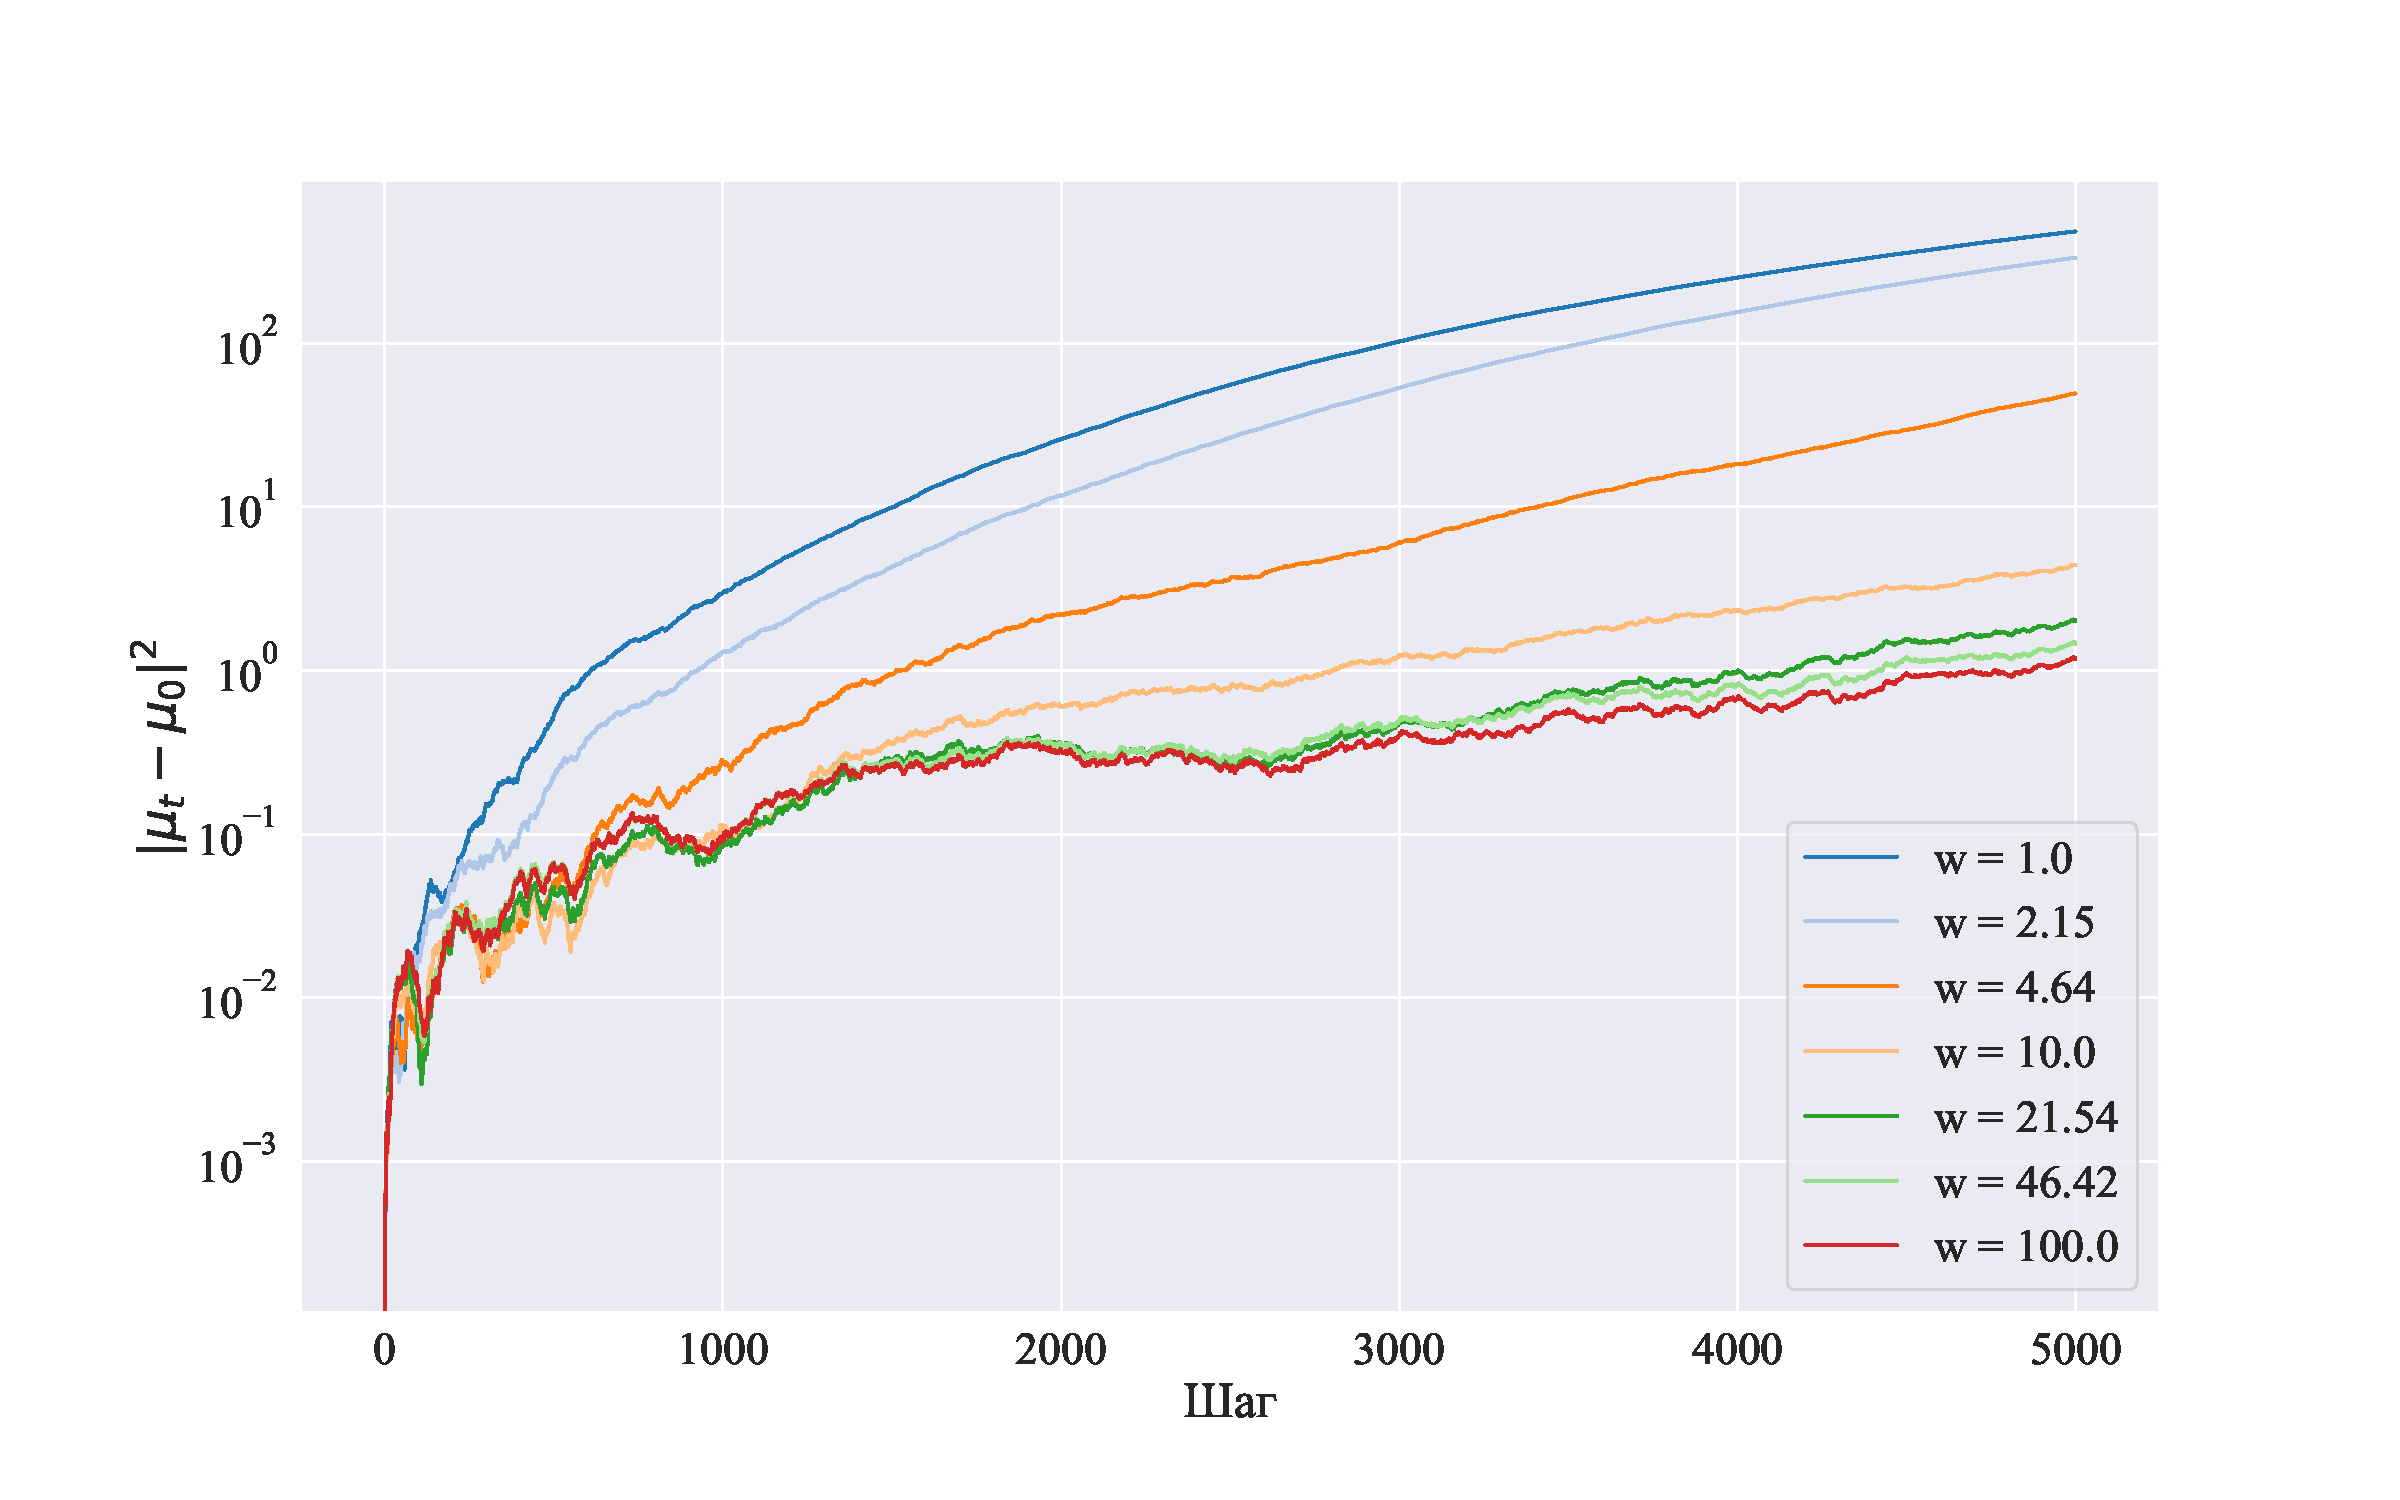
\includegraphics[width=16cm]{norm_interest_random.pdf}
\end{center}
%%%% если имеется doi цитируемого источника, необходимо его указать, см. пример в \bibitem{article}
%%%% DOI публикации, зарегистрированной в системе Crossref, можно получить по адресу http://www.crossref.org/guestquery/
\begin{thebibliography}{99}
\bibitem{webArticle}
    \BibAuthor{Ray~Jiang, Silvia~Chiappa, Tor~Lattimore,Andr{\'a}s Gy{\"o}rgy, Pushmeet~Kohli}
    Degenerate Feedback Loops in Recommender Systems//
    \BibJournal{CoRR}, 2019, Vol. abs/1902.10730,
	  URL: \BibUrl{https://arxiv.org/abs/1902.10730}.

\bibitem{Article}
    \BibAuthor{Khritankov, Anton}
    Hidden Feedback Loops in Machine Learning Systems: A simulation Model and Preliminary Results//
    \BibJournal{Springer}, 2021, P.~54--65,

\bibitem{webArticle}
    \BibAuthor{Daniel Russo, Benjamin Van Roy, Abbas Kazerouni, Ian Osband}
    A Tutorial on Thompson Sampling//
    \BibJournal{CoRR}, 2017, Vol. abs/1707.02038,
	  URL: \BibUrl{https://arxiv.org/abs/1707.02038}.

\bibitem{webArticle}
    \BibAuthor{Shipra Agrawal, Navin Goyal}
    Analysis of Thompson Sampling for the multi-armed//
    \BibJournal{CoRR}, 2011, Vol. abs/1111.1797,
	  URL: \BibUrl{https://arxiv.org/abs/1111.1797}.
\end{thebibliography}

%%%% если имеется doi цитируемого источника, необходимо его указать, см. пример в \bibitem{article}
%%%% DOI публикации, зарегистрированной в системе Crossref, можно получить по адресу http://www.crossref.org/guestquery/.

\end{document}
